\documentclass[12pt]{article}

\usepackage{epsfig,array,amsmath,fancybox,epic}

\usepackage[latin1]{inputenc}

\voffset=-2cm
\hoffset=-1cm

\setlength{\textheight}{25cm}
\setlength{\textwidth}{16cm}
\setlength{\parindent}{0cm}

%-------------------------------------------------------------------------
\setlength{\fboxsep}{3mm}
%-------------------------------------------------------------------------

\begin{document}

\begin{LARGE}
\begin{bf}
\begin{center}
Biblioth\`eque de gestion d'agents
\end{center}
\end{bf}
\end{LARGE}

\vspace{-0.4cm}

\section{Introduction}

\vspace{-0.2cm}

Cette biblioth\`eque de gestion d'agents permet, assez simplement, de
cr\'eer des agents, de les ordonnancer (s\'equentiellement ou
al\'eatoirement) et de permettre la communication entre agents
(point \`a point ou broadcast).

\vspace{0.2cm}
Cette biblioth\`eque est compos\'ee de 3 classes principales~:
\begin{itemize}
\vspace{-0.1cm}
\item[-] {\tt Scheduler} ; la gestion de l'ordonnancement et
du nommage des agents.
\vspace{-0.2cm}
\item[-] {\tt Agent} ; les agents ordonnanc\'es doivent h\'eriter de
cette classe.
\vspace{-0.2cm}
\item[-] {\tt Message} ; les messages \'echang\'es par les agents
doivent h\'eriter de cette classe.
\end{itemize}

Ainsi, un objet de la classe {\tt Scheduler} est charg\'e d'ordonnancer toutes
les instances des classes qui h\'eritent de la classe {\tt Agent}.

\vspace{-0.3cm}
\begin{figure}[hbtp]
\begin{center}
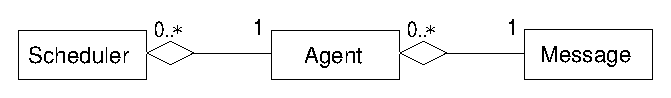
\includegraphics[width=8cm]{fig/UML}
\end{center}
\vspace{-0.8cm}
\caption{Diagramme de classes~: {\tt Scheduler}, {\tt Agent} et {\tt Message}}
\end{figure}

\vspace{-0.2cm}
ATTENTION~:
\begin{itemize}
\vspace{-0.1cm}
\item[-] Un {\tt Scheduler} doit \^etre instanci\'e AVANT les agents qu'il doit
ordonnancer.
\vspace{-0.2cm}
\item[-] Il est toujours pr\'ef\'erable d'instancier un agent dynamiquement
-- via un {\tt new} --.
En effet, cela permet, \`a n'importe quel moment, de supprimer un agent
\`a l'aide d'un {\tt delete}.
Un agent peut ainsi ``se suicider'' ({\tt delete this})
ou ``commettre un meurtre'' en supprimant un autre agent -- connu par son
pointeur --  via un {\tt delete}.
Ainsi, la cr\'eation -- via un {\tt new} -- ou
la suppression -- via un {\tt delete} -- d'un agent peut se faire en cours
de cycle.
\vspace{-0.2cm}
\item[-] Un {\tt Agent} doit poss\'eder une m\'ethode
{\tt void live(double dt)}.
C'est cette m\'ethode qui est appel\'ee cycliquement par l'ordonnanceur.
Si l'ordonnanceur est en mode ``Temps R\'eel'', le param\`etre {\tt dt},
exprim\'e en secondes, correspond au temps \'ecoul\'e depuis la derni\`ere
activation. Sinon, le param\`etre {\tt dt} est \'egal \`a {\tt 0.0}.
\end{itemize}

\vspace{0.1cm}

Exemple~:
\begin{footnotesize}
\label{premierEx}
\begin{verbatim}
#include <iostream>
#include "MAS.h" 
#include "A.h"    // Description de la class A
\end{verbatim}
\begin{verbatim}
using namespace std;
\end{verbatim}
\begin{verbatim}
int main(void)
{
 Scheduler sched;
 sched.setRandomMode(true);       // Passage en ordonnancement aleatoire
 sched.setRealTimeMode(true);     // Passage en mode "temps reel"
\end{verbatim}
\begin{verbatim}
 // Creation de 5 Agents A : "A.1", "A.2", "A.3", "A.4", "A.5"
 for(size_t i=0; i<5 ;i++) { Agent* a = new A;
                             cout << "Creation de " << a->getName() << endl;
 }
\end{verbatim}
\begin{verbatim}
 while (1)         // Execution d'un cycle de simulation :
 {                 // Appel, 1 et 1 seule fois dans le cycle, de la
  sched.cycle();   // methode void live(double dt) de chacun des Agents
 }
\end{verbatim}
\begin{verbatim}
 return 0;    // A la fin, lorsque l'ordonnanceur est detruit, tous les agents
}             // connus par l'ordonnanceur sont automatiquement detruits.
\end{verbatim}
\end{footnotesize}

\newpage

\section{La classe {\tt Agent}}
\vspace{-0.2cm}
Un agent d'une nouvelle classe (classe {\tt A} dans l'exemple
pr\'ec\'edent) doit h\'eriter directement
ou indirectement de la classe {\tt Agent}.
L'interface publique de cette classe {\tt Agent} est la suivante~:

\vspace{-0.3cm}
\begin{footnotesize}
\label{Agent}
\begin{verbatim}
class Agent {
\end{verbatim}
\vspace{-0.5cm}
\begin{verbatim}
 DEFCLASS(Agent)      // Macro liee au nommage des agents
\end{verbatim}
\begin{verbatim}
  friend ostream& operator<<(ostream& os, const Agent& anAgent);
\end{verbatim}
\vspace{-0.6cm}
\begin{verbatim}
 public:
\end{verbatim}
\begin{verbatim}
   // Allocateurs/Desallocateurs
\end{verbatim}
\begin{verbatim}
           Agent(void);
           Agent(const Agent& anAgent);
           Agent& operator=(const Agent& anAgent);
  virtual ~Agent(void);
\end{verbatim}
\begin{verbatim}
  virtual  void live(double dt) {} // dt en seconde: temps depuis la derniere activation
\end{verbatim}
\begin{verbatim}
           void suspend(void);
           void restart(void);
           bool isSuspended(void) const;
\end{verbatim}
\begin{verbatim}
   // Comparaisons
\end{verbatim}
\begin{verbatim}
  friend   bool operator==(const Agent& anAgent1, const Agent& anAgent2);
  friend   bool operator!=(const Agent& anAgent1, const Agent& anAgent2);
\end{verbatim}
\begin{verbatim}
   // Inspecteurs
\end{verbatim}
\begin{verbatim}
           string getName(void) const;  // N'a pas de sens dans le constructeur
           unsigned long getSuffix(void) const; // Idem : n'a pas de sens ...
           string getClass(void) const; // DEFCLASS: virtual getClassName ...
           bool   isA(string aClass) const;
\end{verbatim}
\begin{verbatim}
   // Gestion des messages
\end{verbatim}
\begin{verbatim}
           size_t   getNbMessages(void) const;
           Message* getNextMessage(void); // Le suivant
           void     clearMessageBox(void);
           void     setSensitivity(string aClass,bool yesNo); // Sensibilite (cf broadcast)
   virtual size_t   sendMessageTo(Message& aM,Agent *dest) const; // retourne 1(ok),0(ko)
   virtual void     broadcastMessage(Message& aM) const;
\end{verbatim}
\begin{verbatim}
 protected:
\end{verbatim}
\begin{verbatim}
   // Methodes a appeler par une classe derivee
\end{verbatim}
\begin{verbatim}
                                // Methode qui doit etre appelee dans le constructeur
           void newAgent(void); // d'une classe derivee => Arbre d'heritage
\end{verbatim}
\begin{verbatim}
   //  display a appeler dans une classe derivee       // display est une methode
   virtual void display(ostream& os) const;            // appelee dans operator<<
\end{verbatim}
\begin{verbatim}
   //  isEqualTo a appeler dans une classe derivee     // isEqualTo est une methode
   virtual bool isEqualTo(const Agent& anAgent) const; // appelee dans operator==
};
\end{verbatim}
\end{footnotesize}

Cette classe {\tt Agent} propose les m\'ethodes classiques que
tous les objets C++ doivent avoir (constructeur, constructeur par recopie,
op\'erateur d'affectation, destructeur, op\'erateurs de comparaison,
op\'erateur d'injection dans un flot de sortie pour l'affichage).
De plus, elle propose les m\'ethodes suivantes:

\begin{itemize}
\vspace{-0.2cm}
\item[$\diamond$] De gestion du comportement des agents
\begin{itemize}
\vspace{-0.1cm}
\item[-] {\tt void live(double dt)} ; via une red\'efinition de cette
m\'ethode dans une classe d\'eriv\'ee de la classe {\tt Agent}, il est
possible de sp\'ecifier le comportement associ\'e aux agents de cette
classe d\'eriv\'ee.
\vspace{-0.1cm}
\item[-] {\tt void suspend(void)} ; permet de suspendre le comportement d'un
agent. Sa m\'ethode {\tt live} ne sera plus appel\'ee automatiquement lors
de l'ex\'ecution de la m\'ethode {\tt cycle} de
l'ordonnanceur.
\vspace{-0.1cm}
\item[-] {\tt void restart(void) }; permet de ``relancer'' le comportement
d'un agent.
\vspace{-0.1cm}
\item[-] {\tt bool isSuspended(void)} ; permet de savoir si un agent est
suspendu.
\end{itemize}

\vspace{-0.4cm}
\item[$\diamond$] De gestion des noms d'agents et des classes

\begin{itemize}
\vspace{-0.2cm}
\item[-] {\tt string getName(void)} ; permet d'obtenir le nom d'un agent
(cf nommage des agents). La m\'ethode {\tt getName} n'a pas de sens
dans le constructeur. En effet, dans le constructeur d'une classe,
le nom n'est pas d\'efinitif puisqu'il est, a priori possible, 
de d\'eriver cette classe.
\vspace{-0.1cm}
\item[-] {\tt unsigned long getSuffix(void)} ; permet d'obtenir le suffixe
d'un agent (cf nommage des agents).
Cette m\'ethode n'a pas de sens dans le constructeur.
\vspace{-0.1cm}
\item[-] {\tt string getClass(void)} ; permet d'obtenir le nom de la
classe d'un agent (cf nommage des agents).
\vspace{-0.1cm}
\item[-] {\tt bool isA(string aClass)} ; permet, en prenant en compte
l'arbre d'h\'eritage, de savoir si un agent est un objet d'une classe
particuli\`ere (voir la section \ref{isA}).
\end{itemize}

\vspace{-0.4cm}
\label{boite}
\item[$\diamond$] De gestion de la bo\^ \i te aux lettres des agents
et de l'envoi de messages
%avec des priorit\'es
(voir la classe {\tt Message} d\'ecrite dans la section \ref{Message}).
Signalons que les messages ont une priorit\'e et que la priorit\'e
0 (priorit\'e par d\'efaut) est la priorit\'e la plus faible.
\begin{itemize}
\vspace{-0.2cm}
\item[-] {\tt size\_t getNbMessages(void)} ; permet de conna\^ \i tre
le nombre de messages en attente dans la bo\^ \i te aux lettres
de l'agent.
\vspace{-0.2cm}
\item[-] {\tt Message* getNextMessage(void)} ; permet d'obtenir un
pointeur sur le message suivant (attention, la
destruction du message obtenu (via un pointeur) est \`a la
charge de l'agent... penser \`a faire un delete...!).
\vspace{-0.2cm}
\item[-] {\tt void clearMessageBox(void)} ; vide la bo\^ \i te de
r\'eception.
\vspace{-0.2cm}
\item[-] {\tt void setSensitivity(string aClass,bool yesNo)} ;
permet de rendre sensible l'agent \`a un certain type de
message envoy\'e en broadcast.
\vspace{-0.2cm}
\item[-] {\tt size\_t sendMessageTo(Message\& aM,Agent *dest)} ; permet
d'envoyer un message \`a un agent particulier.\\
Retourne {\tt 1} si ok, {\tt 0} si l'envoi n'est pas possible
(i.e. l'agent {\tt dest} n'existe pas).
\vspace{-0.6cm}
\item[-] {\tt void broadcastMessage(Message\& aM)} ; permet
d'envoyer un message en broadcast (les agents sensibles au(x) type(s)
du message envoy\'e recevront alors le message).
\end{itemize}
\end{itemize}

\vspace{-0.3cm}

La classe {\tt Agent} comporte \'egalement les m\'ethodes {\tt protected}~:
\begin{itemize}
\vspace{-0.2cm}
\item[-] {\tt virtual void display(ostream\& os)} ; cette m\'ethode
appel\'ee par l'{\tt operator<<} permet d'afficher un agent.
\vspace{-0.2cm}
\item[-] {\tt virtual bool isEqualTo(const Agent\& anAgent)} ; cette
m\'ethode appel\'ee par la fonction amie {\tt operator==} permet
de tester l'\'egalit\'e de deux agents.
\end{itemize}

%\vspace{-0.15cm}

Ainsi on a~:
\begin{footnotesize}
\begin{verbatim}
ostream& operator<<(ostream& os,const Agent& anAgent)
{
 anAgent.display(os);
 return os;
}
\end{verbatim}
\end{footnotesize}
et
\vspace{-0.15cm}
\begin{footnotesize}
\begin{verbatim}
bool operator==(const Agent& anAgent1, const Agent& anAgent2)
{
 return anAgent1.isEqualTo(anAgent2);
}
\end{verbatim}
\end{footnotesize}

L'int\'er\^et principal de ces deux m\'ethodes {\tt display} et
{\tt isEqualTo} est que l'on peut facilement les red\'efinir dans
les classes d\'eriv\'ees de la classe {\tt Agent}.

\vspace{0.2cm}

Ainsi, si l'on reprend l'exemple de la classe {\tt A} qui h\'erite
de la classe {\tt Agent}, on peut \'ecrire~:
\begin{footnotesize}
\begin{verbatim}
void A::display(ostream& os) const
{
 Agent::display(os);              // Affichage de la partie Agent de A

 ...      // Affichage des attributs propres a un objet de la classe A
}
\end{verbatim}
\end{footnotesize}
\vspace{-0.15cm}
et
\vspace{-0.15cm}
\begin{footnotesize}
\begin{verbatim}
bool A::isEqualTo(const A& anA) const
{
 ...    // Test de l'egalite des attributs propres a un objet de la classe A

 if (!(Agent::isEqualTo(anA))) return false; // Test de la partie Agent de A
 return true;
}
\end{verbatim}
\end{footnotesize}

Maintenant, si l'on consid\`ere une classe {\tt B}, qui h\'erite de la
classe {\tt A}, ces 2 m\'ethodes peuvent \^etre red\'efinies ainsi~:
\begin{footnotesize}
\begin{verbatim}
void B::display(ostream& os) const
{
 A::display(os);             // Affichage de la partie A de l'object B

 ...      // Affichage des attributs propres a un objet de la classe B
}
\end{verbatim}
\end{footnotesize}
\vspace{-0.15cm}
et
\vspace{-0.15cm}
\begin{footnotesize}
\begin{verbatim}
bool B::isEqualTo(const B& aB) const
{
 ...    // Test de l'egalite des attributs propres a un objet de la classe B

 if (!(A::isEqualTo(aB))) return false;  // Test de la partie A de l'objet B
 return true;
}
\end{verbatim}
\end{footnotesize}


{\bf AUTRE METHODE DE LA CLASSE {\tt Agent}~:} {\tt void newAgent(void)}

\vspace{0.2cm}

Cette m\'ethode ne doit pas \^etre red\'efinie.
Elle doit juste \^etre imp\'erativement appel\'ee dans les constructeurs
des classes d\'erivant (directement ou non) de la classe {\tt Agent}.

Cette m\'ethode {\tt newAgent} de la classe {\tt Agent} sert en effet
au nommage des agents.
L'absence d'appel \`a cette fonction dans les constructeurs peut
entra\^ \i ner des incoh\'erences au niveau du nom des agents.

\vspace{0.2cm}

{\bf ATTENTION~:} cette m\'ethode {\tt newAgent} est fortement li\'ee
\`a la macro {\tt DEFCLASS} dont un appel doit se trouver dans la
d\'eclaration de la classe. 
Ainsi, dans la d\'eclaration de la classe {\tt Agent}
(voir page \pageref{Agent}),
nous pouvons voir l'appel suivant~: {\tt DEFCLASS(Agent)}.
De la m\^eme fa\c con, dans la d\'eclaration d'une classe {\tt A},
il doit y avoir l'appel suivant~: {\tt DEFCLASS(A)}... Et la m\^eme
chose pour une classe {\tt B}, etc...

\vspace{0.2cm}
A titre d'illustration d'utilisation de {\tt newAgent},
si l'on reprend l'exemple de la classe {\tt A} qui h\'erite
de la classe {\tt Agent}, les 2 constructeurs de cette classe {\tt A}
doivent appeler la m\'ethode {\tt newAgent}~:

\begin{footnotesize}
\begin{verbatim}
A::A(void) : Agent()
{
 newAgent();
}
\end{verbatim}
\begin{verbatim}
//--
A::A(const A& anA) : Agent(anA)
{
 newAgent();
 ...         // Copie a effectuer pour la classe A
}
\end{verbatim}
\end{footnotesize}

Maintenant, si l'on consid\`ere une classe {\tt B}, qui h\'erite de la
classe {\tt A}, les 2 constructeurs de cette classe {\tt B}
doivent \'egalement appeler la m\'ethode {\tt newAgent}~:

\begin{footnotesize}
\begin{verbatim}
B::B(void) : A()
{
 newAgent();
}
\end{verbatim}
\begin{verbatim}
//--
B::B(const B& aB) : A(aB)
{
 newAgent();
 ...         // Copie a effectuer pour la classe B
}
\end{verbatim}
\end{footnotesize}

\subsection{Exemple~: une classe A h\'eritant de la classe {\tt Agent}}

Soient le fichier {\tt A.h} suivant~:

\begin{footnotesize}
\begin{verbatim}
#ifndef _A_H_            /////////////// A.h ///////////////
#define _A_H_
\end{verbatim}
\begin{verbatim}
#include <iostream>
#include "MAS.h"
\end{verbatim}
\begin{verbatim}
using namespace std;
\end{verbatim}
\begin{verbatim}
class A : public Agent
{
  DEFCLASS(A)
\end{verbatim}
\begin{verbatim}
  friend ostream& operator<<(ostream& os, const A& anA);
\end{verbatim}
\begin{verbatim}
 public :
\end{verbatim}
\begin{verbatim}
   // Allocateurs/Desallocateurs
\end{verbatim}
\begin{verbatim}
            A(void);
            A(const A& anA);
            A& operator=(const A& anA);
   virtual ~A(void);
\end{verbatim}
\newpage
\begin{verbatim}
   virtual  void live(double dt);

   // Comparaisons

   friend  bool operator==(const A& anA1, const A& anA2);
   friend  bool operator!=(const A& anA1, const A& anA2);

   // Inspecteurs/modificateurs

 protected :

   // Methodes a appeler par une classe derivee

   // display: a appeler dans une classe derivee      // display est une
   virtual void display(ostream& os) const;           // methode appelee
                                                      // dans operator<<

   // isEqualTo: a appeler dans une classe derivee (dans operator==)
   virtual bool isEqualTo(const A& anA) const;

 private :

   // Methodes privees d'allocation/desallocation

   void _copy(const A& anA);
   void _destroy(void);
};

#endif // _A_H_
\end{verbatim}
\end{footnotesize}

et le fichier {\tt A.cpp} suivant~:

\begin{footnotesize}
\begin{verbatim}
#include "A.h"           ////////////// A.cpp //////////////

//--
A::A(void) : Agent()
{
 newAgent();
}

//--
A::A(const A& anA) : Agent(anA)
{
 newAgent();
 _copy(anA);
}

//--
A& A::operator=(const A& anA)
{
 if (this != &anA)
 {
  Agent::operator=(anA);
  _destroy();
  _copy(anA);
 }
 return *this;
}

//--
A::~A(void)
{
 _destroy();
}

//--
void A::live(double dt)
{
 // "Comportement" d'un Agent de la classe A
 cout << "A::My name is " << getName() << endl;
}

//--
bool operator==(const A& anA1, const A& anA2)
{
 return anA1.isEqualTo(anA2);
}

//--
bool operator!=(const A& anA1, const A& anA2)
{
 return !(anA1==anA2);
}

//--
ostream& operator<<(ostream& os, const A& anA)
{
 anA.display(os);
 return os;
}

//--
void A::display(ostream& os) const
{
 Agent::display(os);
 // Affichage des attributs de la classe A (Ici, pas d'attribut dans A!)
}

//--
bool A::isEqualTo(const A& anA) const
{
 // Test des attributs de la classe A (Ici, pas d'attribut dans A!)
 if (!(Agent::isEqualTo(anA))) return false;
 return true;
}

//--
void A::_copy(const A& anA)
{
 // Affectation des attributs de la classe A (Ici, pas d'attribut dans A!)
}

//--
void A::_destroy(void)
{
 // Destruction des attributs de la classe A (Ici, pas d'attribut dans A!)
}
\end{verbatim}
\end{footnotesize}

\subsection{Exemple~: une classe B h\'eritant de la classe {\tt A}}

Soient le fichier {\tt B.h} suivant~:

\begin{footnotesize}
\begin{verbatim}
#ifndef _B_H_            /////////////// B.h ///////////////
#define _B_H_

#include <iostream>

#include "MAS.h"
#include "A.h"

using namespace std;

class B : public A
{
  DEFCLASS(B)

  friend ostream& operator<<(ostream& os, const B& aB);

 public :

   // Allocateurs/Desallocateurs

            B(void);
            B(const B& aB);
            B& operator=(const B& aB);
   virtual ~B(void);

   virtual  void live(double dt);

   // Comparaisons

   friend  bool operator==(const B& aB1, const B& aB2);
   friend  bool operator!=(const B& aB1, const B& aB2);

   // Inspecteurs/modificateurs

 protected :

   // Methodes a appeler par une classe derivee

   // display: a appeler dans une classe derivee      // display est une
   virtual void display(ostream& os) const;           // methode appelee
                                                      // dans operator<<

   // isEqualTo: a appeler dans une classe derivee (dans operator==)
   virtual bool isEqualTo(const B& aB) const;

 private :

   // Methodes privees d'allocation/desallocation

   void _copy(const B& aB);
   void _destroy(void);
};

#endif // _B_H_
\end{verbatim}
\end{footnotesize}

\newpage

et le fichier {\tt B.cpp} suivant~:

\begin{footnotesize}
\begin{verbatim}
#include "B.h"           ////////////// B.cpp //////////////
//--
B::B(void) : A()
{
 newAgent();
}

//--
B::B(const B& aB) : A(aB)
{
 newAgent();
 _copy(aB);
}

//--
B& B::operator=(const B& aB)
{
 if (this != &aB)
 {
  A::operator=(aB);
  _destroy();
  _copy(aB);
 }
 return *this;
}

//--
B::~B(void)
{
 _destroy();
}

//--
void B::live(double dt)
{
 // Comportement" d'un Agent de la classe B
 cout << "B::My name is " << getName() << endl;
}

//--
bool operator==(const B& aB1, const B& aB2)
{
 return aB1.isEqualTo(aB2);
}

//--
bool operator!=(const B& aB1, const B& aB2)
{
 return !(aB1==aB2);
}

//--
ostream& operator<<(ostream& os, const B& aB)
{
 aB.display(os);
 return os;
}
\end{verbatim}
\begin{verbatim}
//--
void B::display(ostream& os) const
{
 A::display(os);
 // Affichage des attributs de la classe B (Ici, pas d'attribut dans B!)
}
\end{verbatim}
\vspace{-0.6cm}
\begin{verbatim}
//--
bool B::isEqualTo(const B& aB) const
{
 // Test des attributs de la classe B (Ici, pas d'attribut dans B!)
 if (!(A::isEqualTo(aB))) return false;
 return true;
}
\end{verbatim}
\vspace{-0.6cm}
\begin{verbatim}
//--
void B::_copy(const B& aB)
{
 // Affectation des attributs de la classe B (Ici, pas d'attribut dans B!)
}
\end{verbatim}
\vspace{-0.6cm}
\begin{verbatim}
//--
void B::_destroy(void)
{
 // Destruction des attributs de la classe B (Ici, pas d'attribut dans B!)
}
\end{verbatim}
\end{footnotesize}

\section{Nommage des agents et gestion des instances}

Nous avons vu dans la section pr\'ec\'edente consacr\'ee \`a la
classe {\tt Agent} que les agents avaient un nom.

Encore une fois, cette fonctionnalit\'e est possible gr\^ace~:
\begin{itemize}
\item[-] \`a l'appel \`a la macro {\tt DEFCLASS} dans chaque d\'eclaration
de classe h\'eritant (directement ou non) de la classe {\tt Agent} ;
\item[-] \`a l'appel \`a la fonction {\tt newAgent} dans chaque
constructeur de classe h\'eritant (directement ou non) de la classe
{\tt Agent}.
\end{itemize}

Si l'on respecte bien les appels \`a {\tt DEFCLASS} et \`a {\tt newAgent},
le nom d'un agent est une cha\^ \i nes de caract\`eres compos\'ee
du nom de la classe de l'agent suivi d'un num\'ero d'instance.

Ainsi, la premi\`ere instance d'une classe {\tt A} aura comme nom "A.1",
la deuxi\`eme "A.2", etc...

Le suffixe d'un agent (voir la m\'ethode {\tt getSuffix})
correspond \`a son num\'ero d'instance.

\subsection{Rappels sur la classe {\tt Agent}}

Gestion des noms d'agents et des classes dans la classe {\tt Agent}~:

\begin{itemize}
\vspace{-0.2cm}
\item[-] {\tt string getName(void)} ; permet d'obtenir le nom d'un agent.
Rappel: la m\'ethode {\tt getName} n'a pas de sens dans le constructeur. 
En effet, dans le constructeur d'une classe, le nom n'est pas d\'efinitif
puisqu'il est, a priori possible, de d\'eriver cette classe.
\item[-] {\tt unsigned long getSuffix(void)} ; permet d'obtenir le suffixe
d'un agent.
Cette m\'ethode n'a pas de sens dans le constructeur.
\item[-] {\tt string getClass(void)} ; permet d'obtenir le nom de la
classe d'un agent.
\item[-] {\tt bool isA(string aClass)} ; permet, en prenant en compte
l'arbre d'h\'eritage, de savoir si un agent est un objet d'une classe
particuli\`ere
(dans l'exemple pr\'ec\'edent avec les classes {\tt A} et {\tt B},
un appel \`a la m\'ethode {\tt isA} sur une instance de la
classe {\tt B} retourne {\tt true} si le param\`etre
pass\'e \`a {\tt isA} est {\tt "Agent"}, {\tt "A"} ou {\tt "B"}.
\end{itemize}

\vspace{0.3cm}

\subsection{Fonctionnalit\'es de gestion des noms et des instances}

\vspace{0.3cm}

La librairie de gestion d'agents fournit \'egalement quelques services
concernant la gestion des instances.

Ainsi, les fonctions sont disponibles~:
\begin{itemize}
\vspace{0.1cm}
\item[-] {\tt void getAllAgents(string aClass,
           vector<Agent*>\& anAgentVector)} ;
cette fonction permet d'obtenir dans un vecteur STL la
liste des agents appartenant \`a une classe donn\'ee
(l'arbre d'h\'eritage \'etant pris en compte~:
dans l'exemple pr\'ec\'edent avec les classes {\tt A} et {\tt B},
un appel \`a {\tt getAllAgents} avec comme premier
param\`etre {\tt "A"} donne toutes les instances de {\tt A} mais aussi
celles de {\tt B}).
\vspace{0.1cm}
\item[-] {\tt Agent* getAgent(string aName)} ;
cette fonction permet, connaissant un nom d'agent, d'obtenir
un pointeur sur cet agent.
\vspace{0.1cm}
\item[-] {\tt bool exist(const Agent* anAgent)} ; 
cette fonction permet, connaissant un pointeur sur un agent,
de savoir si cet agent existe encore... 
\end{itemize}

Remarque~: {\tt getAllAgents}, {\tt getAgent} et {\tt exist}
sont des fonctions...

\hspace{2.25cm}...pas des m\'ethodes de classe~!

\subsection{Un point sur la m\'ethode
{\tt isA} de la classe {\tt Agent}}
\label{isA}

La m\'ethode {\tt bool isA(string aClass)} de la classe {\tt Agent}
permet, en prenant en compte l'arbre d'h\'eritage, de savoir si un
agent est un objet d'une classe particuli\`ere.

Concr\`etement, 
connaissant un pointeur sur un {\tt Agent},
l'id\'ee est ici de savoir si l'agent ``point\'e'' est un objet
d'une classe d\'eriv\'ee particuli\`ere.

\vspace{0.3cm}

{\bf Exemple d'utilisation}

\begin{itemize}
\item[-] Soit {\tt Agt} une classe d\'eriv\'ee de la classe {\tt Agent}.
\item[-] Soient {\tt A} et {\tt B} deux classes d\'eriv\'ees de la
classe {\tt Agt}.
\end{itemize}

Le morceau de programme suivant permet~:

\begin{itemize}
\item[-] de r\'ecup\'erer des pointeurs
sur tous les agents de la classe de base {\tt Agt}
(c'est--\`a--dire,
des agents de la classe {\tt Agt},
des agents de la classe {\tt A}
et des agents de la classe {\tt B})~;

\item[-] d'appliquer un traitement
particulier en fonction des classes
effectives des agents ``point\'es''.

\end{itemize}

\begin{footnotesize}
\begin{verbatim}

...
vector<Agent*> v;
...
getAllAgents("Agt",v);
...
for(size_t i=0;i<v.size();i++)
{
 Agent* agent=v[i];

 if (agent->isA("A")) { 
                        A* a=(A*)agent: 
                        a->doSomethingsForA();   // Traitement particulier pour A
 }
 else
 if (agent->isA("B")) { 
                        B* b=(B*)agent: 
                        b->doSomethingsForB();   // Traitement particulier pour B
 }
 else
 {
  Agt* agt=(Agt*)agent:
  agt->doSomethingsForAgt();                     // Traitement particulier pour Agt
 }
}
...
\end{verbatim}
\end{footnotesize}

\section{La classe {\tt Scheduler}}

\vspace{0.3cm}

L'instanciation d'un objet de la classe {\tt Scheduler}
est indispensable au bon fonctionnement d'une application
multi--agents.

\begin{footnotesize}
\begin{verbatim}
class Scheduler
{
 public:

  // Allocateurs/Desallocateurs

                     Scheduler(void);
  // Non implemente: Scheduler(const Scheduler& aScheduler);
  // Non implemente: Scheduler& operator=(const Scheduler& aScheduler);
            virtual ~Scheduler(void);

                void cycle(void);

                void setRandomMode(bool randomMode);
                bool getRandomMode(void) const;

                void setRealTimeMode(bool realTimeMode);
                bool getRealTimeMode(void) const;
};
\end{verbatim}
\end{footnotesize}

L'utilisation classique d'un ordonnanceur a \'et\'e pr\'esent\'ee
lors du premier exemple (voir page \pageref{premierEx}).

\newpage

Ainsi, nous pouvons r\'esumer les diff\'erentes grandes \'etapes
de la cr\'eation d'une application multi-agents~:

\vspace{-0.3cm}
\begin{footnotesize}
\begin{verbatim}
...
int main(void)
{
 Scheduler sched;     // Instanciation d'un ordonnanceur
\end{verbatim}
\begin{verbatim}
 sched.setRandomMode(true);     // Passage eventuel en ordonnancement aleatoire
 sched.setRealTimeMode(true);   // Passage eventuel en mode "temps reel"
\end{verbatim}
\vspace{-0.8cm}
\begin{verbatim}
 ... // Instanciation dynamique des agents presents au debut de la simulation
\end{verbatim}
\vspace{-0.8cm}
\begin{verbatim}
 while (1)
 {                 // Execution d'un cycle de simulation :
  sched.cycle();   // Appel, 1 et 1 seule fois dans le cycle, de la
                   // methode void live(double dt) de chacun des Agents
  vector<Agent*> v;
  getAllAgents("Agent",v);
  if (v.size()==0) break;    // Ou bien une condition plus simple... ou pas de condition!
 }
\end{verbatim}
\vspace{-0.8cm}
\begin{verbatim}
 return 0;   // A la fin, lorsque l'ordonnanceur est detruit, tous les agents
}            // connus par l'ordonnanceur sont automatiquement detruits.
\end{verbatim}
\end{footnotesize}

Un ordonnanceur poss\`ede donc les m\'ethodes suivantes~:
\begin{itemize}
\vspace*{-0.2cm}
\item[-] {\tt setRandomMode(bool randomMode)} ; permet de fixer le
mode d'activation (s\'equen\-tiel ou al\'eatoire) des agents.
Si {\tt randomMode} est {\tt true}, activation du mode al\'eatoire.
Sinon, activation du mode s\'equentiel.
\vspace*{-0.2cm}
\item[-] {\tt bool getRandomMode(void)} ; permet de r\'ecup\'erer
le mode d'activation (s\'equentiel ou al\'eatoire) li\'e \`a l'ordonnanceur.
\vspace*{-0.2cm}
\item[-] {\tt setRealTimeMode(bool realTimeMode)} ; permet de fixer le
mode ``temps r\'eel'' ou non.
Si {\tt realTimeMode} est {\tt true}, activation du mode ``temps r\'eel''.
Sinon activation du mode non ``temps r\'eel''.
\vspace*{-0.2cm}
\item[-] {\tt bool getRealTimeMode(void)} ; permet de r\'ecup\'erer
le mode (``temps r\'eel'' ou non) li\'e \`a l'ordonnanceur.
\vspace*{-0.2cm}
\item[-] {\tt void cycle(void)} ; permet de faire ``vivre'' une et une
seule fois un agent... c'est \`a dire, ex\'ecuter un cycle de simulation.
Le mode est s\'equentiel ou al\'eatoire, ``temps r\'eel'' ou non, en
fonction des r\'eglages faits avec {\tt setRandomMode} et
{\tt setRealTimeMode}.
\end{itemize}

Remarque importante~: s'il y a plusieurs {\tt Scheduler} instanci\'es,
les agents sont tous ordonnanc\'es par le premier {\tt Scheduler} ayant
\'et\'e instanci\'e~ (l'``ordonnanceur courant'')~!

\vspace{-0.3cm}
\section{La classe {\tt Message}}
\label{Message}

\vspace{-0.1cm}
Nous avons vu que les agents pouvaient s'\'echanger des messages.
Tous les messages \'echang\'es entre les agents doivent h\'eriter
(directement ou non) de la classe {\tt Message}.

Les messages ont une priorit\'e. La priorit\'e
0 (priorit\'e par d\'efaut) est la priorit\'e la plus faible.
Plus la priorit\'e associ\'ee \`a un message est \'elev\'ee, plus
le message est prioritaire.

\vspace{0.2cm}

Comme pour la classe {\tt Agent}, il existe des contraintes sur l'\'ecriture
du code {\tt C++}. Ainsi~:
\begin{itemize}
\vspace{-0.2cm}
\item[-] Dans la d\'eclaration d'une classe correspondant \`a un
nouveau type de message, il doit y avoir un appel \`a la
macro {\tt DEFCLASS}.
\vspace{-0.2cm}
\item[-] Dans les constructeurs des classes h\'eritant (directement ou non)
de la classe {\tt Message}, il doit y avoir un appel \`a la m\'ethode
{\tt newMessage} de cette m\^eme classe {\tt Message}.
\end{itemize}

Ces deux appels sont indispensables au bon fonctionnement des
\'echanges de messages.

Un message doit donc h\'eriter directement
ou indirectement de la classe {\tt Message}.
L'inter\-fa\-ce publique de cette classe {\tt Message} est la suivante~:

\vspace{0.2cm}

\begin{footnotesize}
\begin{verbatim}
class Message {

 DEFCLASS(Message)    // Pour le bon fonctionnement ...

  friend ostream& operator<<(ostream& os, const Message& aMessage);

 public:

   // Allocateurs/Desallocateurs

           Message(void);
           Message(const Message& aMessage);
           Message& operator=(const Message& aMessage);
  virtual ~Message(void);

           void   setPriority(size_t priority);
           size_t getPriority(void) const;

   // Comparaisons

  friend   bool operator==(const Message& aMessage1, const Message& aMessage2);
  friend   bool operator!=(const Message& aMessage1, const Message& aMessage2);

   // Inspecteurs

           string getClass(void)   const; // DEFCLASS: virtual getClassName ...
           bool   isA(string aClass) const;
           Agent* getEmitter(void) const; // Avant l'envoi d'un message,
                                          // l'emetteur est NULL ...!

 protected:

   // Methodes a appeler par une classe derivee

                                // Methode qui doit etre appelee dans le cons-
         void newMessage(void); // tructeur d'une classe derivee
                                // => Arbre d'heritage

   //  display a appeler dans une classe derivee        // display est une
   virtual void display(ostream& os) const;             // methode appelee
                                                        // dans operator<<

   //  isEqualTo a appeler dans une classe derivee      // isEqualTo est une
   virtual bool isEqualTo(const Message& aMessage) const; // methode appelee
                                                          // dans operator==

};
\end{verbatim}
\end{footnotesize}

Cette classe {\tt Message} propose les m\'ethodes classiques que
tous les objets C++ doivent avoir (constructeur, constructeur par recopie,
op\'erateur d'affectation, destructeur, op\'era\-teurs de comparaison,
op\'erateur d'injection dans un flot de sortie pour l'affichage).

\newpage

La classe {\tt Message} propose \'egalement les m\'ethodes suivantes:

\begin{itemize}
\vspace{-0.2cm}
\item[-] {\tt void   setPriority(size\_t priority) }; permet de fixer
la priorit\'e associ\'ee \`a un message. 
La priorit\'e 0 (priorit\'e par d\'efaut) est la priorit\'e la plus faible.
Plus la priorit\'e associ\'ee \`a un message est \'elev\'ee, plus
le message est prioritaire.
\item[-] {\tt size\_t getPriority(void)} ; permet d'obtenir la priorit\'e
associ\'ee \`a un message.
\item[-] {\tt string getClass(void)} ; permet d'obtenir le nom de la
classe d'un message.
\item[-] {\tt bool isA(string aClass)} ; permet, en prenant en compte
l'arbre d'h\'eritage, de savoir si un message est un objet d'une classe
particuli\`ere.
\item[-] {\tt Agent* getEmitter(void)} ; permet de conna\^ \i tre
l'agent ayant envoy\'e le message.\\
Attention~: l'\'emetteur d'un message n'est disponible qu'une fois
le message envoy\'e..!
\end{itemize}

La classe {\tt Message} poss\`ede \'egalement des m\'ethodes
tr\`es similaires \`a celles disponibles dans la classe {\tt Agent}. 
Ainsi, la classe {\tt Message} comporte \'egalement les m\'ethodes
{\tt protected}~:
\begin{itemize}
\item[-] {\tt virtual void display(ostream\& os)} ; cette m\'ethode
appel\'ee par l'{\tt operator<<} permet d'afficher un message.
\vspace{-0.2cm}
\item[-] {\tt virtual bool isEqualTo(const Message\& aMessage)} ; cette
m\'ethode appel\'ee par la fonction amie {\tt operator==} permet
de tester l'\'egalit\'e de deux messages.
\end{itemize}

Comme nous l'avons d\'ej\`a indiqu\'e, la classe {\tt Message} poss\`ede
\'egalement une m\'ethode {\tt newMessage} fortement li\'ee
\`a la macro {\tt DEFCLASS} dont un appel doit se trouver dans la
d\'eclaration de la classe.

Cette m\'ethode {\tt void newMessage(void)} ne doit pas \^etre red\'efinie.
Elle doit juste \^etre imp\'erativement appel\'ee dans les constructeurs
des classes d\'erivant (directement ou non) de la classe {\tt Message}.

Cette m\'ethode {\tt newMessage} sert \`a cr\'eer l'arbre d'h\'eritage
entre messages.
L'absence d'appel \`a cette fonction dans les constructeurs peut
entra\^ \i ner des incoh\'erences au niveau des envois de messages.

\vspace{-0.2cm}
\subsection{Envoi/R\'eception de message par un agent}

Un agent a \`a sa disposition un certain nombre de m\'ethodes
(voir page \pageref{boite}) lui permettant
de g\'erer sa bo\^ \i tes aux lettres, d'envoyer un message \`a un agent
particulier, de se rendre sensibles \`a certains types de messages \'emis
en broadcast et, enfin, d'envoyer en broadcast un message aux agents
sensibles au(x) type(s) du message envoy\'e (en prenant en compte
l'arbre d'h\'eritage des messages).

\vspace{-0.2cm}
\subsection{Un point sur la m\'ethode
{\tt isA} de la classe {\tt Message}}

La m\'ethode {\tt isA} de la classe {\tt Message} permet \`a
un {\tt Agent} de g\'erer simplement sa bo\^ \i te \`a messages
m\^eme si des messages de diff\'erents types y sont stock\'es.

\vspace{0.3cm}

{\bf Exemple d'utilisation}

\begin{itemize}
\item[-] Soient {\tt MA} et {\tt MB} deux classes d\'eriv\'ees de la
classe {\tt Message}.
\end{itemize}

Le morceau de programme suivant permet \`a un agent de type
{\tt UneClasseAgent} de lire sa bo\^ \i te \`a messages
en distingant les messages de type {\tt MA} et ceux de type {\tt MB}.

\begin{footnotesize}
\begin{verbatim}
void UneClasseAgent::live(double dt)
{
 ...
 while (getNbMessages())
 {
  Message* m = getNextMessage();

  if (m->isA("MA") { MA* ma=(MA*)m;
                     // Utilisation, via le pointeur ma, du message de type MA
  }
  else
  if (m->isA("MB") { MB* mb=(MB*)m;
                     // Utilisation, via le pointeur mb, du message de type MB
  }

  delete m; // Important pour eviter les "fuites" memoire
 }
 ...
}
\end{verbatim}
\end{footnotesize}

\section{G\'en\'erateur de code pour les classes {\tt Agent} et {\tt Message}}

\vspace{0.5cm}

Afin de simplifier le travail du programmeur, un g\'en\'erateur de classes
d\'erivant de {\tt Agent} ou de {\tt Message} a \'et\'e r\'ealis\'e.

\vspace{0.2cm}
Il se trouve dans le r\'epertoire~: {\tt Generateurs}.
et s'utilise de la fa\c con suivante~:

\vspace{0.2cm}
{\tt \$ ./genere Agent} pour cr\'eer une classe d\'erivant (directement
ou non) de {\tt Agent}

\vspace{0.2cm}
ou bien

\vspace{0.2cm}
{\tt \$ ./genere Message} pour cr\'eer une classe d\'erivant (directement
ou non) de {\tt Message}

\vspace{0.2cm}
Dans les deux cas, le nom de la classe est demand\'e ainsi que
le nombre de classes d\'eriv\'ees... et les noms de ces classes.
Le g\'en\'erateur cr\'ee alors un fichier {\tt .h} et un fichier {\tt .cpp}.

\vspace{0.2cm}
Le g\'en\'erateur fournit un squelette minimal permettant de cr\'eer
une nouvelle classe...
Les parties \`a modifier (arguments du constructeur, ...) sont rep\'er\'ees
dans le code \`a l'aide de {\tt \#\#\#}.

\vspace{0.5cm}
{\bf ... C'est bien pratique !}

\hspace{0.5cm}{\bf ... C'est bien pratique !}

\hspace{1cm}{\bf ... C'est bien pratique !}

\hspace{1.5cm}{\bf ... C'est bien pratique !}

\hspace{2cm}{\bf ... C'est bien pratique !}

\hspace{2.5cm}{\bf ... C'est bien pratique !}

\hspace{3cm}{\bf ... C'est bien pratique !}

\hspace{3.5cm}{\bf ... C'est bien pratique !}

\hspace{4cm}{\bf ... C'est bien pratique !}

\hspace{4.5cm}{\bf ... C'est bien pratique !}

\hspace{5cm}{\bf ... Et en plus j'ai encore de la place !}

\newpage

\section{A savoir: quelques fonctions utilitaires}

La biblioth\`eque de gestion d'{\tt Agent} fournit \'egalement quelques
fonctions utilitaires concernant la gestion du temps et la gestion
de nombres al\'eatoires~:

\vspace{-0.1cm}
\begin{center}
voir le fichier {\tt LibMoRis/include/UtilAgent.h}
\end{center}

\vspace{-0.2cm}
\begin{itemize}
\item Gestion du temps~:
\begin{itemize}
\item {\tt double getTimeMicroSeconds(void);}\\
retourne le temps courant en microsecondes.
\vspace{-0.1cm}
\item {\tt double getTimeMilliSeconds(void);}\\
retourne le temps courant en millisecondes.
\vspace{-0.1cm}
\item {\tt double getTimeSeconds(void);}\\
retourne le temps courant en secondes.
\end{itemize}
\vspace{-0.2cm}
\item Gestion de nombres al\'eatoires~:
\begin{itemize}
\item {\tt void~~~initRandom(void);}\\
initialise le g\'en\'erateur de nombres al\'eatoires.
\vspace{-0.1cm}
\item {\tt size\_t~randomMinMax(size\_t min, size\_t max);}\\
permet d'obtenir un nombre entier positif compris entre {\tt min} et {\tt max}.
\vspace{-0.1cm}
\item {\tt double~random01(void);}\\
permet d'obtenir un nombre r\'eel compris entre~{\tt 0}~et~{\tt 1}.
\end{itemize}
\end{itemize}

\section{Bugs connus}

Sous Cygwin, le mode temps r\'eel ne fonctionne probablement pas
correctement \`a cause d'un bug connu de la fonction
{\tt gettimeofday}...

Pour essayer de rem\'edier \`a ce probl\`eme j'ai ajout\'e
une attente -- {\tt usleep(1);} -- juste avant l'appel
\`a {\tt gettimeofday}.... voir le fichier {\tt UtilAgent.cpp}.

Bien s\^ur, cet ajout se fait uniquement lorsque l'on compile
{\tt UtilAgent.cpp} sous Cygwin~!

\section{A faire un jour}

\begin{itemize}
\item[-] Utiliser des ``smart pointers'' pour g\'erer les messages...
permet d'\'eviter de recopier un message avant qu'il ne soit
mis dans la bo\^ \i te aux lettres d'un agent.
\item[-] Revoir la m\'ethode d'ordonnancement
({\tt Scheduler::cycle(void)}) et \'evaluer les performances lorsque
beaucoup d'agent doivent \^etre g\'er\'es.
\end{itemize}

\section{A savoir sur l'h\'eritage multiple\\
pour programmeurs avertis...}

Afin de faire de l'h\'eritage multiple~:
\begin{itemize}
\item[-] dans la classe {\tt Agent}, il y a la m\'ethode
{\tt void newAgent(Agent* This);}
\vspace{-0.3cm}
\item[-] dans la classe {\tt Message}, il y a la m\'ethode
{\tt void newMessage(Message* This);}
\end{itemize}

Pour l'utilisation de l'h\'eritage multiple,
voir les exemples se trouvant ici~:
\begin{center}
{\tt GestionAgents/Exemples/ExemplesPourProgrammeursAvertis/HeritageMultiple}
\end{center}

\newpage

\section{A savoir sur la classe {\tt Scheduler}...\\
pour programmeurs avertis...\\
pour faire des SMA de SMA}

En r\'ealit\'e, la classe {\tt Scheduler} comporte en plus de ce qui
a \'et\'e annonc\'e~:
\begin{itemize}
\item Un constructeur par recopie et l'op\'erateur d'affectation

$\Longrightarrow$ la copie d'un ordonnanceur {\tt o} dans un autre
ordonnanceur implique la copie des agents ordonnanc\'es par
l'ordonnanceur {\tt o}.

\item Des m\'ethodes permettant de g\'erer/modifier
l'``ordonnanceur courant''.
Le terme ``ordonnanceur courant'' doit \^etre compris ici comme
l'ordonnanceur auquel est automatiquement rattach\'e un agent lorsque
celui-ci est instanci\'e.
\end{itemize}

\noindent
Pour avoir acc\`es \`a ces nouvelles fonctionnalit\'es,
la ligne num\'ero 4 du fichier
\begin{center}
{\tt GestionAgents/LibMoRis/include/Scheduler.h}
\end{center}
doit \^etre d\'e-comment\'ee~!... Et la biblioth\`eque
re-compil\'ee.

\begin{center}
{\tt //\#define SMAdeSMA} $\Longrightarrow$ {\tt \#define SMAdeSMA}
\end{center}

\begin{footnotesize}
\begin{verbatim}
class Scheduler
{
 public:

   // Allocateurs/Desallocateurs

                     Scheduler(void);
                     Scheduler(const Scheduler& aScheduler); // Progr. avertis!
                     Scheduler& operator=(const Scheduler& aScheduler); // Idem
            virtual ~Scheduler(void);

                void cycle(void);

                void setRandomMode(bool randomMode);
                bool getRandomMode(void) const;

                void setRealTimeMode(bool realTimeMode);
                bool getRealTimeMode(void) const;

   // Gestion de plusieurs ordonnanceurs
   //-- Pour programmeurs avertis ... pour faire des SMA de SMA !
   //
   //-- Constructeur par recopie et affectation
   // Implemente !    Scheduler(const Scheduler& aScheduler);
   // Implemente !    Scheduler& operator=(const Scheduler& aScheduler);
   //
   //-- Changement et memorisation de l'ordonnanceur courant........
    static void       setCurrentSched(Scheduler& aScheduler);
    static void       setCurrentSched(Scheduler* aSchedulerPtr);
    static Scheduler* getCurrentSched(void);
   //
};
\end{verbatim}
\end{footnotesize}

Pour l'utilisation de plusieurs ordonnanceurs,
voir l'exemple se trouvant ici~:
\begin{center}
{\tt GestionAgents/Exemples/ExemplesPourProgrammeursAvertis/SMAdeSMA}
\end{center}

\newpage

\section{A savoir sur la classe {\tt Agent}...\\
pour programmeurs avertis...\\
pour changer la m\'ethode automatiquement \\
activ\'ee par l'ordonnanceur..........................!}

Jusqu'\`a pr\'esent, nous avons vu que, pour une classe {\tt A} qui
h\'erite de la classe {\tt Agent}, l'ordonnanceur appelle automatiquement
la m\'ethode {\tt void A::live(double dt);} de chacune des instances
de cette classe {\tt A}.

\vspace{0.3cm}

Ceci peut \^etre modifi\'e tr\`es simplement car,
en r\'ealit\'e, la classe {\tt Agent} comporte en plus de ce qui
a \'et\'e annonc\'e~:
\begin{itemize}
\item {\tt void setLiveMethod(liveMethodType newLiveMethod);}
\item {\tt liveMethodType getLiveMethod(void);}
\end{itemize}

O\`u le type {\tt liveMethodType} correspond \`a la d\'efinition
d'un nouveau type\\
``Pointeur sur des m\'ethodes activables par l'ordonnanceur'':
\begin{center}
{\tt typedef void (Agent::*liveMethodType)(double dt);}
\end{center}

\vspace{0.3cm}

La m\'ethode {\tt void Agent::setLiveMethod(liveMethodType newLiveMethod);}
permet, pour une instance donn\'ee, de changer la m\'ethode qui sera
automatiquement appel\'ee par l'ordonnanceur.

\vspace{0.1cm}

La m\'ethode {\tt liveMethodType Agent::getLiveMethod(void);} permet
de r\'ecup\'erer un pointeur sur la m\'ethode actuellement appel\'ee
automatiquement pour une instance donn\'ee.

\vspace{0.3cm}
Exemple d'utilisation de la m\'ethode {\tt setLiveMethod}:
\begin{itemize}
\item Soit une classe {\tt A} ayant une m\'ethode
{\tt void A::behavior(double dt);}
\item Soit {\tt A *a = new A( avec d'\'eventuels param\`etres );} 
\item L'appel {\tt a->setLiveMethod((liveMethodType)\&A::behavior);}
aura pour cons\'e\-quen\-ce que, pour l'instance {\tt a}, l'ordonnanceur
appelera automatiquement la m\'ethode {\tt A::behavior}
\end{itemize}

Remarques:
\begin{itemize}
\item Si le param\`etre pass\'e \`a {\tt setLiveMethod} est {\tt NULL},
c'est le comportement par d\'efaut qui est remis.
Ainsi, par la suite, la m\'ethode {\tt live} sera appel\'ee automatiquement
par l'ordonnanceur.
\item Au cours de la vie d'une instance, ce n'est pas n\'ecessairement
toujours la m\^eme m\'ethode qui sera appel\'ee automatiquement pas
l'ordonnanceur... puisque, \`a tout moment, avec un appel \`a
{\tt setLiveMethod}, il est possible de changer de m\'ethode~!

\end{itemize}

\vspace{0.5cm}

Pour l'utilisation sur un exemple complet de ces nouvelles m\'ethodes
de la classe {\tt Agent},\\
voir l'exemple se trouvant ici~:
\vspace{-0.5cm}
\begin{center}
{\tt GestionAgents/Exemples/ExemplesPourProgrammeursAvertis/Exemple\_setLiveMethod}
\end{center}


\ifnum 1 = 1
\newpage
\section{Fichier {\tt MAS.h}}

Ce fichier reprend les diff\'erents {\tt .h} et fonctions
utiles...

\begin{footnotesize}
\begin{verbatim}
                    
#ifndef _MAS_H_
#define _MAS_H_


//%%%%%%%%%%%%%%%%%%%%%  MACRO DEFCLASS  %%%%%%%%%%%%%%%%%%%%%%%%%%%

#define DEFCLASS(className) \
private: virtual string getClassName(void) const\
{ \
  return #className; \
} \
private : virtual void* virtualCopy(void) const \
{ \
 return (void*)new className(*this); \
}

//%%%%%%%%%%%%%%%%%%%%%%%%%%%%%%%%%%%%%%%%%%%%%%%%%%%%%%%%%%%%%%%%%%

class Agent;
class Scheduler;
class Message;

#include "Agent.h"
#include "Message.h"
#include "Scheduler.h"

#include "UtilAgent.h"

extern void   getAllAgents(string aClass, vector<Agent*>& anAgentVector);
extern Agent* getAgent(string aName);
extern bool   exist(const Agent* anAgent);

\end{verbatim}
%\newpage
\begin{verbatim}
/* 

*******************************   Utilities  (UtilAgent.h) *****************

///////////////////////////// Gestion du temps ///////////////////////////////

extern double getTimeMicroSeconds(void);               // En microsecondes
extern double getTimeMilliSeconds(void);               // En millisecondes
extern double getTimeSeconds(void);                    // En secondes

///////////////////////////// Generation aleatoire //////////////////////////

extern void   initRandom(void);                    // Initialisation generateur
extern size_t randomMinMax(size_t min, size_t max);// Generation dans [min,max]
extern double random01(void);                      // Generation dans [0.0,1.0]

/////////////////////////////////////////////////////////////////////////////

\end{verbatim}
\newpage
\begin{verbatim}
*******************************  class Agent (Agent.h) *********************
\end{verbatim}
\vspace{-0.5cm}
\begin{verbatim}
typedef void (Agent::*liveMethodType)(double dt); // Pour get/setLiveMethod...
\end{verbatim}
\vspace{-0.5cm}
\begin{verbatim}
class Agent {
\end{verbatim}
\vspace{-0.5cm}
\begin{verbatim}
 DEFCLASS(Agent)
\end{verbatim}
\vspace{-0.5cm}
\begin{verbatim}
  friend ostream& operator<<(ostream& os, const Agent& anAgent);
\end{verbatim}
\begin{verbatim}
 public:
\end{verbatim}
\vspace{-0.5cm}
\begin{verbatim}
   // Allocateurs/Desallocateurs
\end{verbatim}
\vspace{-0.5cm}
\begin{verbatim}
           Agent(void);
           Agent(const Agent& anAgent);
           Agent& operator=(const Agent& anAgent);
  virtual ~Agent(void);
\end{verbatim}
\vspace{-0.5cm}
\begin{verbatim}
  virtual  void live(double dt)               // dt en seconde : temps depuis
           {                                  // la derniere activation
            // Rien pour un Agent de base
            (void)dt;  // Pour eviter un warning
           }
\end{verbatim}
\vspace{-0.5cm}
\begin{verbatim}
           void suspend(void);
           void restart(void);
           bool isSuspended(void) const;
\end{verbatim}
\vspace{-0.5cm}
\begin{verbatim}
           void setLiveMethod(liveMethodType newLiveMethod); // Progr. avertis!
           liveMethodType getLiveMethod(void);               // Progr. avertis!
\end{verbatim}
\vspace{-0.5cm}
\begin{verbatim}
   // Comparaisons
\end{verbatim}
\vspace{-0.5cm}
\begin{verbatim}
  friend   bool operator==(const Agent& anAgent1, const Agent& anAgent2);
  friend   bool operator!=(const Agent& anAgent1, const Agent& anAgent2);
\end{verbatim}
\vspace{-0.5cm}
\begin{verbatim}
   // Inspecteurs
\end{verbatim}
\vspace{-0.5cm}
\begin{verbatim}
           string getName(void) const;  // N'a pas de sens dans le constructeur 
           unsigned long getSuffix(void) const; // Idem : n'a pas de sens ...
           string getClass(void) const; // DEFCLASS: virtual getClassName ... 
           bool   isA(string aClass) const;
\end{verbatim}
\vspace{-0.5cm}
\begin{verbatim}
   // Gestion des messages
\end{verbatim}
\vspace{-0.5cm}
\begin{verbatim}
           size_t   getNbMessages(string aClass="Message") const;
           Message* getNextMessage(string aClass="Message"); // Le suivant
           void     clearMessageBox(void);
\end{verbatim}
\vspace{-0.5cm}
\begin{verbatim}
           void     setSensitivity(string aClass,bool yesNo);
                                                                 // retourne
   virtual size_t   sendMessageTo(Message& aM,Agent *dest) const;// 1(ok),0(ko)
   virtual void     broadcastMessage(Message& aM) const;
\end{verbatim}
\vspace{-0.5cm}
\begin{verbatim}
 protected:
\end{verbatim}
\vspace{-0.5cm}
\begin{verbatim}
   // Methodes a appeler par une classe derivee
\end{verbatim}
\vspace{-0.5cm}
\begin{verbatim}
                                 // Methode qui doit etre appelee dans le constructeur
           void newAgent(void);  // d'une classe derivee => Arbre d'heritage
           void newAgent(Agent* This); // Idem mais pour l'heritage multiple
\end{verbatim}
\vspace{-0.5cm}
\begin{verbatim}
   //  display a appeler dans une classe derivee       // display est une methode
   virtual void display(ostream& os) const;            // appelee dans operator<<
\end{verbatim}
\vspace{-0.5cm}
\begin{verbatim}
   //  isEqualTo a appeler dans une classe derivee     // isEqualTo est une
   virtual bool isEqualTo(const Agent& anAgent) const; // methode appelee
};                                                     // dans operator==
\end{verbatim}
\newpage
\begin{verbatim}
******************************  class Message (Message.h) ******************
\end{verbatim}
\begin{verbatim}
class Message {
\end{verbatim}
\begin{verbatim}
 DEFCLASS(Message)
\end{verbatim}
\begin{verbatim}
  friend ostream& operator<<(ostream& os, const Message& aMessage);
\end{verbatim}
\begin{verbatim}
 public:
\end{verbatim}
\begin{verbatim}
   // Allocateurs/Desallocateurs
\end{verbatim}
\begin{verbatim}
           Message(void);
           Message(const Message& aMessage);
           Message& operator=(const Message& aMessage);
  virtual ~Message(void);

           void   setPriority(size_t priority);
           size_t getPriority(void) const;
\end{verbatim}
\begin{verbatim}
   // Comparaisons
\end{verbatim}
\begin{verbatim}
  friend   bool operator==(const Message& aMessage1, const Message& aMessage2);
  friend   bool operator!=(const Message& aMessage1, const Message& aMessage2);
\end{verbatim}
\begin{verbatim}
   // Inspecteurs
\end{verbatim}
\begin{verbatim}
           string getClass(void)   const; // DEFCLASS: virtual getClassName ...
           bool   isA(string aClass) const;
           Agent* getEmitter(void) const; // Avant l'envoi d'un message,
                                          // l'emetteur est NULL ...!
 protected:
\end{verbatim}
\begin{verbatim}
   // Methodes a appeler par une classe derivee
\end{verbatim}
\begin{verbatim}
                                // Methode qui doit etre appelee dans le constructeur
         void newMessage(void); // d'une classe derivee => Arbre d'heritage
         void newMessage(Message* This); // Idem mais pour l'heritage multiple
\end{verbatim}
\begin{verbatim}
   //  display a appeler dans une classe derivee        // display est une
   virtual void display(ostream& os) const;             // methode appelee
                                                        // dans operator<<
\end{verbatim}
\begin{verbatim}
   //  isEqualTo a appeler dans une classe derivee      // isEqualTo est une
   virtual bool isEqualTo(const Message& aMessage) const; // methode appelee
                                                          // dans operator==
};
\end{verbatim}
\newpage
\begin{verbatim}
*****************************  class Scheduler (Scheduler.h) ***************

class Scheduler
{

 public:

 // Allocateurs/Desallocateurs

                     Scheduler(void);
                     Scheduler(const Scheduler& aScheduler); // Progr. avertis!
                     Scheduler& operator=(const Scheduler& aScheduler); // Idem
            virtual ~Scheduler(void);

                void cycle(void);

                void setRandomMode(bool randomMode);
                bool getRandomMode(void) const;

                void setRealTimeMode(bool realTimeMode);
                bool getRealTimeMode(void) const;

  //-- Gestion de plusieurs ordonnanceurs...
  //-- Pour programmeurs avertis ... pour faire des SMA de SMA !
  //
  //-- Constructeur par recopie et affectation
  // Implemente !    Scheduler(const Scheduler& aScheduler);
  // Implemente !    Scheduler& operator=(const Scheduler& aScheduler);
  //
  //-- Changement et memorisation de l'ordonnanceur courant........
   static void       setCurrentSched(Scheduler& aScheduler);
   static void       setCurrentSched(Scheduler* aSchedulerPtr);
   static Scheduler* getCurrentSched(void);
  //
};

*/

#endif // _MAS_H_
\end{verbatim}
\end{footnotesize}
\fi

\newpage

\section{Installation}

\vspace{1cm}

\begin{figure}[hbtp]
\begin{center}
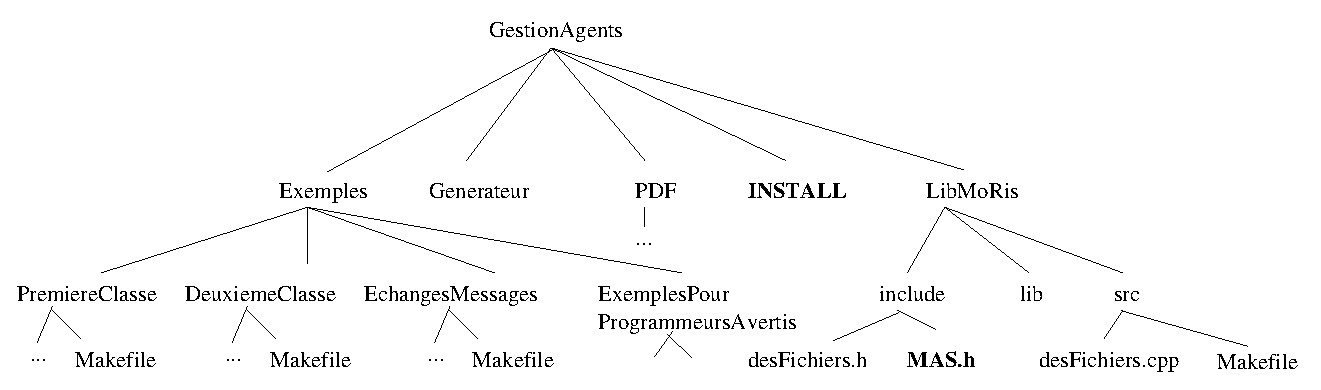
\includegraphics[width=15.5cm]{fig/arbo}
\end{center}
\caption{Description de l'arborescence de la biblioth\`eque}
\end{figure}

Aller dans le r\'epertoire {\tt LibMoRis/src}
et faire {\tt \$ make}

Une biblioth\`eque {\tt libAgents.a} est alors plac\'ee dans le r\'epertoire
{\tt LibMoRis/lib}

Des exemples de programmes sont disponibles dans le r\'epertoire
{\tt Exemples}.

\vspace{0.5cm}
{\bf ... mais on peut faire plus simple !}

\vspace{0.5cm}

En \'etant dans le r\'epertoire {\tt GestionAgents}, faire tout
simplement {\tt \$ ./INSTALL}

Il faut ensuite aller dans les r\'epertoires avec les divers exemples
et faire {\tt \$ make}

\end{document}
